\graphicspath{{8/figures/}}
\chapter{Conclusion}
\label{chp:conclusion}

This thesis has explored the application of deep learning methods to the general domain of automatic music description, focusing on timbre similarity and automatic chord estimation.
Encouraging performance is obtained in both areas, advancing the state of art in the latter, while providing deeper insight to the tasks at hand.
These observations encourage the slight reformulation of chord estimation as a representation learning, rather than a classification, problem, resulting in a high performing system with myriad practical benefits.
This chapter summarizes the main contributions of this work, and offers perspectives for the future, including an assessment of outstanding challenges and the potential impact of continued research in this domain.

\section{Summary}

Automatic music description is at the heart of content-based music informatics research.
This is necessary for problems where manual annotation does not scale, such as acoustic similarity, as well as problems where most people lack the musical expertise to perform the task well, such as transcription.
While this topic is independently valuable, it would seem that progress is decelerating, and thus any efforts to correct this course must first determine why.
In Chapter \ref{chp:context}, common practice in automatic music description was revisited, leading to the identification of three deficiencies worth addressing:
hand-crafted feature design is not sustainable, shallow architectures are fundamentally limited, and short-time analysis alone fails to capture long-term musical structure.
Deep architectures and feature learning were shown to hold promise in music analysis tasks, evidenced both conceptually and by its growing success, motivating the exploration of deep learning in automatic music description.

At this point, it was necessary to consider what is ``deep learning'', and why is this an option now?
In Chapter \ref{chp:deep_learning}, the history of the field was first re-examined, showing that after an over-hyped introduction, neural networks languished through the latter part of the 20th century.
This period of skepticism and disinterest gave technology time to catch up to the theory, and after a series of significant research contributions, deep learning made a triumphant return to the fore of computer science, toppling longstanding benchmarks seemingly overnight.
While this has brought about a second wave of hype and interest, it also encouraging the curation of a more established theory of deep networks.
As reviewed, the modern practice of deep learning consists of a handful of modular processing blocks, strung together in differentiable functions and numerically optimized to an objective function via gradient-based methods, complemented by a growing suite of practical tricks of the trade.

Having reviewed the modern core of deep learning, this work shifted focus in Chapter \ref{chp:timbre} to explore these methods directly.
As a first inquiry, a deep convolutional network was applied to the task of timbre similarity, achieving three goals:
the model is able to learn relevant signal-level features that give rise to source identification;
the resulting output space is organized in a semantically meaningful way;
and the smoothness of the space is indicated by error analysis.
The approach presented here also offers novel extensions to previous efforts in pairwise training, achieving extremely robust representations despite a considerable reduction in dimensionality.
And perhaps most importantly, these results are obtained without the need for costly subjective pairwise ratings of content.

Whereas timbre similarity served as a relatively constrained problem, Chapter \ref{chp:chord_estimation} sought to test the limits of deep learning as applied to automatic chord estimation, a well-established music informatics challenge.
Competitive performance is achieved with a deep convolutional neural network, evaluated in both a conventional and large-vocabulary variant of the task.
Somewhat more interestingly, rigorous error analysis reveals that efforts in automatic chord estimation are converging to a glass ceiling, due in large part to the objective formulation of an often subjective experience.
The problems caused by the tenuous nature of ``ground truth'' annotations are exacerbated by efforts to treat chord estimation as a flat, rather than hierarchical, classification task.
Therefore, the single most critical advancement facing the topic of automatic chord estimation is a re-evaluation of the task the community is attempting to solve and the data used to do so.

Despite these difficulties, the chord estimation data is leveraged to ask a slightly different question: can a model be built to automatically predict chords as guitar tablature?
Therefore, in Chapter \ref{chp:guitar}, again using a deep convolutional architecture, global performance statistics are improved over the general chord estimation system, while offering significant practical benefits.
In addition to being a high-performing system, the fretboard estimations are immediately human-readable and thus attractive from a user experience perspective.
Such a representation is also advantageous from a data collection, correction, and validation standpoints, significantly reducing the degree of prerequisite skill necessary to contribute annotations.

Finally, the various open source software artifacts developed in the course of this research are introduced and detailed in Chapter \ref{chp:reproducibility}:
\texttt{jams}, the structured music annotation format designed for multiplicity of both annotator perspective and task namespace;
\texttt{biggie}, an approach to managing large collections of numerical data for training stochastic learning algorithms;
\texttt{optimus}, a user-friendly library for describing and serializing trainable processing graphs;
\texttt{mir\_eval}, a suite of evaluation tools for benchmarking music description algorithms;
and finally \texttt{dl4mir}, a common framework for the systems and results presented here.


\section{Perspectives on Future Work}
\label{sec:future}

Based on the work performed herein and observations made in the process, this section offers several perspectives on deep learning, music informatics, and the intersection between them, in the spirit of helping guide future work.


\subsection{Architectural Design in Deep Learning}

Among the most common questions currently facing the application of deep learning to any problem is that of architectural design.
``How many layers,'' one might ask, ``or how many kernels are necessary for this to work?
Should I use convolutions, or matrix products, or something else altogether?
And furthermore, if and when it does actually work, what on earth is it doing?''
Admittedly, the combination of numerical optimization and extremely versatile functions often results in systems with opaque mid-level representations, earning deep networks the reputation as ``black boxes'' and the study of them a ``dark art''.
However, while these enigmatic functions might cause understandable confusion, the design of deep architectures is not necessarily devoid of intuition.

% Simply train the systems we've already got
But where to start?
The simplest way one might begin to explore deep learning for some problem of choice is to build some previously published algorithm and use gradient descent to fine-tune the hand crafted weights.
There are countless MIR systems that can and are being reformulated in the deep learning framework, such as onset detection, instrument identification, or pitch estimation.
Most importantly, doing so eliminates the need to compare minor implementation details, like specific hyperparameters or window coefficients;
just learn it and let it all come out in the wash.
Additionally, introducing the process of learning to classic music informatics systems makes it easier to \emph{combine} multiple systems to reap the benefits of model averaging.
The key takeaway here is the notion that good architectures already exist for some problems, and that better performance can be obtained by using numerical optimization to expand the space of parameters considered.

% Or explore new ones
Critically, these lessons and practices transcend known problems to new ones.
As demonstrated with the fretboard architecture of Chapter \ref{chp:guitar}, systems can be quickly constructed by appropriately constraining the behavior.
Since a guitar has six strings, and each can only be active in one place, it makes sense to model each as a probability surface.
That said, there is much more that could be done here.
Perhaps transition constraints could be imposed, such that the model would prefer common chord shapes, or positional constraints, whereby nearby frets are preferred to large jumps.
In this manner, end-to-end systems can be designed and developed at a high level, and numerical optimization can be leveraged to work out the fine details.
Furthermore, while learning can discover useful features that were previously overlooked or not considered, this advantage is amplified for new challenges and applications that do not offer much guiding intuition.
For tasks like artist identification or automatic mixing, it is difficult to comprehend, much less articulate, exactly what signal attributes are informative to the task and how an implementation might robustly capture this information.

% Abstraction
Thus, deep learning, as an approach to system design, transforms the challenge from ``how do I \emph{implement} the desired behavior?'' to ``how do I \emph{achieve} the desired behavior?''
The nature of this advantage is illustrated by the relationship between programming in a high-level language, like Python, and a low-level one, like assembly.
Technically speaking, both can be used to the same ends, but high-level languages allow for faster development of complex systems by abstracting away the minute details, like memory management or the laborious task of moving data around registers.
% Knowledge of low-level operation is often critical to success in its higher level counterpart, but powerful languages do not absolve the developer of design.
In both cases, precise control is traded for power, leaving the developer to focus on the task at hand with greater speed and efficiency.
Note, however, that abstraction doesn't eliminate the need for sound architecture, only the need to worry about certain facets.
The fundamental design challenge is the same, but operating at a higher level of abstraction allows the deep learning researcher to build bigger systems faster.

% Takeaway: it's not really guess work, there's still work to be done.
Therefore, it is worthwhile to note that music informatics researchers are quite proficient at leveraging domain knowledge, engineering acumen, and a bit of intuition to architect signal processing systems;
how many principal components should one keep of a feature representation?
what is a suitable window size for a Fourier transform?
how many subbands should a given filterbank have?
The same intuition can and should be used to design deep networks, as discussed in the learning of chroma, the design of a tempo estimation system, or constructing instrument-specific models.
% Digital signal theory is still relevant,
Ultimately, the process of designing a deep architecture is as arbitrary or intentional as one makes it; it's only guesswork if you're guessing.


\subsection{Practical Advice for Fellow Practitioners}

%
While the previous discussion hopefully serves to address some of the mystery inherent to deep learning, it certainly entails the disclaimer of ``your mileage may vary.''
The following are a handful of guidelines accumulated in the course of research;
far more suggestion than direction, they have served well in practice.

\begin{enumerate}

\item \textbf{Data is fundamental}:
The data-driven researcher will live and die by the quality of data available.
It is widely held that lots of weakly labeled data will often trump a small amount of strongly labeled data.
The cousin of this sentiment is once you have enough data, everything will come out in the wash.
Take care to note that though this may hold for training, with caveats, the inverse is true for evaluation.
Furthermore, beware obscure biases in data.
Greedy optimization will happily yield bad solutions because of oversights in the curation of training data.
This is particularly true of regression problems.
It is possible to compensate for biased data in classification via uniform class presentation or likelihood scaling, but this can be far less obvious for continuous valued outputs.


\item \textbf{Design what you know, learn what you don't}:
As mentioned, neural networks offer the theoretical promise of the universal approximation theorem, but realizing such general behavior is far from trivial.
It is therefore crucial to leverage domain knowledge where possible.
This will typically take two forms:
one, simplify the learning problem by removing degrees of freedom known to be irrelevant to the problem;
two, constrain the learning problem to encourage musically plausible solutions.
If loudness doesn't impact one's ability to recognize chords, for example, the data should probably be normalized.
Music informatics researchers have a diverse background on which to draw, and this knowledge can be incorporated into the model or training strategy.
Notably, curriculum learning ---the process by which data presented during training are ordered as a function of some variable, e.g. difficulty--- will likely become a much larger topic in the near future, and much can be incorporated from music education and pedagogy in this process.
For example, a data-driven approach to rhythm analysis might first attempt to recognize simple patterns before moving on syncopation and polyrhythms, rather than attempt to make sense of all content at once.


\item \textbf{Over-fitting is your friend}:
Long heralded as the boon of deep networks, over-fitting is arguably a \emph{good} sign, and far more desirable behavior than the inverse.
Simply put, if a deep network is unable to over-fit the training data, something is likely wrong.
This is often due to one or more of the following three issues;
one, it is indicative of a problem with the data, e.g. the observations and targets are uncorrelated or, worse, conflicting;
two, the chosen model lacks the representational power to fit the training data;
or three, and most problematic, the learning problem is poorly posed and optimization is getting stuck in a bad local minima.
The methods for dealing with such issues are not so well codified, but consist of data cleaning, exploring ``bigger'' models, unsupervised pre-training, changing the loss function, etc.; that said, the efficacy of such approaches will vary case by case.


\item \textbf{Get good mileage out of greedy optimization}:
Gradient descent and other such greedy methods are certainly prone to bad local minima, but it is not impossible to take active measures to discourage unfortunate solutions.
% Encourage good behaviour and discourage the bad.
Additionally, it may be easier to define the kinds of things a model \emph{shouldn't} do than the things it should.
For example, a fretboard prediction network could incorporate a penalty whereby ``unplayable'' chord shapes incur significant loss to help keep outputs in a realistic space.


\item \textbf{The gap between ``real'' and synthetic music is closing}:
As more modern music transitions to a digital environment, the difference in quality between a purely acoustic sound recording and one synthesized for research purposes is continually decreasing.
Generally speaking, samplers, synthesizers, and other music production software are increasingly prevalent in modern popular music, but largely underutilized in data-driven music research.
These high quality tools can also be used for data augmentation to make algorithms robust to irrelevant deformations, such as perceptual codecs, background noise, tempo modulation, or pitch shifting.
By generating an unprecedented amount of realistic training data, can we functionally solve tasks such as onset detection, pitch detection, or tempo estimation?

\end{enumerate}


\subsection{Limitations, Served with a Side of Realism}

% Part of a larger arc
As some of its forebears recognize and advocate, especially those who persevered through the first AI winter, it is crucial to maintain reasonable expectations for what can be achieved with deep learning.
Shown in Figure \ref{fig:deephype}, it is interesting to consider that, to date, the path of deep learning has roughly followed Gartner's hype cycle for emerging technologies:
after a most promising start followed by a period of disinterest, neural networks have sharply returned to prominence.

\begin{figure}
\begin{centering}
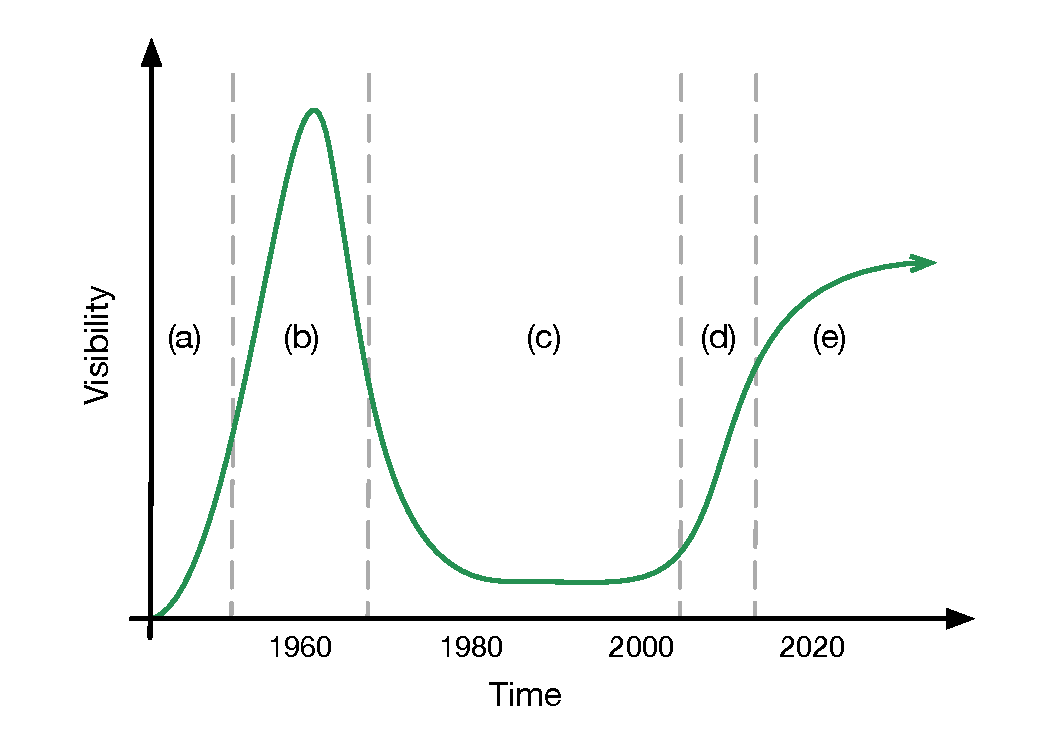
\includegraphics[width=0.6\textwidth]{deephype}
\caption{Gartner Hype cycle, applied to the trajectory of neural networks, consisting of five phases: (a) innovation, (b) peak of inflated expectations, (c) trough of disillusionment, (d) slope of enlightenment, and (e) plateau of productivity.}
\label{fig:deephype}
\end{centering}
\end{figure}

% Deep learning is trending
It goes almost without saying that excitement and interest in deep learning is spiking across computer science, in academia and industry alike.
Research groups are forming based primarily on deep learning, it is being used to win increasing number of data science competitions, and the topic has become common fodder for popular science articles and interviews.
With all the success and attention, it is easy to get carried away in thinking that deep learning is the proverbial ``magic bullet'', that it might topple all problems in due time.

The reality, however, is far more modest.
Deep learning \emph{is} indeed several important things.
It is a powerful approach to non-linear system design.
Deep networks make fantastic models of physical phenomena, and could have profound use in the fields of acoustics, immersive audio, or amplifier modeling.
It is extremely versatile, and can be easily adapted in application-specific ways that other powerful machines, such as SVMs, cannot.
And, given significant gains in compute power, the combination of architectural flexibility and numerical optimization makes it an arguably efficient research strategy, at least more so than graduate students manually tuning parameters.

That said, there are a few important things deep learning is not.
It is by no means the best answer to every problem.
Deep learning is, in its current forms, still relatively data hungry and often computationally expensive.
Even in the case of unsupervised pre-training, sufficient volumes of realistic data may not be trivial to obtain, as in the case of accelerometers or gyroscopes for use in musically oriented human-computer interaction research.
To the latter point, any performance gains obtained with a deep network could be effectively negated by disproportionate increase in processing time.
Both of these limitations are like to become less important over time, but remain relevant today.
More conceptually, albeit somewhat contentiously, nor can the modern flavors of deep learning be called ``intelligent'';
echoing the ghost of John Searle, a system may certainly \emph{behave} intelligently without truly \emph{being} so.
Despite the imagery evoked by metaphors and figurative language that pervade the field, deep learning has as much in common with humanity as a player piano, and learning is merely a means of programming in a data-driven manner.
This is not to say that deep learning can or will not lead to such breakthroughs, but care should be taken when differentiating metaphor from reality.

% Takeaways:
What should one make of deep learning then?
Suffice it to say that deep learning is just another tool ---a powerful tool, but a tool nonetheless--- to be included in the toolbelt of the information science practitioner.
Similar to the trajectories of other, now standard, methods, such as principal components analysis, Gaussian mixture models, or support vector machines, deep learning is settling into the final stage of its hype cycle, the point at which it becomes a means to solve a problem.
\emph{Is deep learning some magic bullet?}
Of course not.
\emph{Is it intelligent?}
Hardly.
But is it useful?
Can it accelerate the process of system design and implementation?
Can it allow the clever researcher to quickly vet ideas and develop complex, robust systems?
The answer to all of these is \emph{yes}.


\subsection{A Handful of Possible Next Steps}

In the course of this thesis, several possible opportunities for subsequent research have been identified.
Here, an effort is made to consolidate the bigger ideas into a single list, as well as introduce other observations gleaned during the research process.

First, there are a variety of specific ways in which the work on timbre similarity could be easily extended.
Based on visual inspection alone, more diffuse embeddings are probably necessary to achieve a strong sense of perceptual smoothness.
One likely way this could be achieved is by limiting similarity during training to intra-class near-neighbors, rather than all observations from a given class.
To this point, a perceptual study would prove enlightening as a means of better understanding what, if any, salient dimensions are captured by the model.
Additionally, in the space of user experience, it would be valuable to better assess the usefulness of these embeddings for a visual-based search for sounds.
In a creative vein, timbre ``morphing'' could be realized by defining a trajectory through an embedding space, and using concatenative synthesis on short-time windows of the corresponding audio signals.
More generally though, this approach could be expanded to consider other kinds of audio or music data, such as vocals, chord labels, or urban environmental sounds.

On the topic of chords and harmony, a few tasks for future research have also been identified.
One, a better definition of the problem is necessary in order to make substantive progress.
As a result, this will make it necessary to reconsider and, in all likelihood, expand the music content used for development and evaluation.
In order to embrace subjectivity, it will be important to additionally collect multiple perspectives on chord labels whenever possible.
This more nuanced reference signal will provide more stable evaluation, while allowing researchers to tackle chord labeling as a tagging problem using a harmonic vocabularity.
From a system design perspective, the relationship with music structure analysis and boundary detection are obvious, and a more explicit fusion of approaches would almost certainly prove fruitful.
Finally, and arguably of greatest importance, one or more automatic chord estimation systems desperately need to be evaluated by a large number of real users, and the findings disseminated within the community.
This is critical to not only validate or redefine our objective measures, but also identify and prioritize deficiencies in modern ACE systems.

Complementing the discussion of general chord estimation above, there are specific extensions to the work on guitar chord tablature worth exploring.
It is a particular limitation of the current system that only single chord voicings are represented, and support for multiple chord shapes would lead to a more expressive system.
Furthermore, more effort could be made to decode the fretboard estimations in physically plausible ways, as in the work of Burlet \cite{Burlet2013Robotaba}.
Given the initial impetus for this work, though, the most valuable action to take next would be to deploy the system via an online application.
This both serves the previous goal of collecting feedback on the quality of the system, as well as allowing users to correct errors, thus growing the amount the labeled data for training and evaluation of future systems.
Furthermore, this speaks to an observation that encompasses all music informatics research:
there is a great deal to be gained by deploying even moderately performing systems as a means of facilitating data collection.
Traditionally, the process of annotating music for curating ground truth is achieved entirely by manual means, and less-than-perfect algorithms can be leveraged to greatly accelerate this daunting task.
The merits of this approach have been aptly demonstrated with the success of reCAPTCHA and its role in optical character recognition research.

Outside the scope of the specific applications tackled in this work, there are a number of other ways in which deep learning can be applied to music informatics.
Perhaps most simply, gradient-based optimization is a viable approach to tweak and tune previous developed algorithms.
Many complex systems, such as instrument recognition, melody tracking, or tempo estimation, can be reinterpreted as deep, differentiable architectures, allowing parameters to be tuned automatically, rather than heuristically.
Approaching problems through the lens of deep learning does not require abandoning previous research in favor of these trendy new methods;
rather, our collective progress serves as a starting point from which data-driven development can take these systems to the next level.
Furthermore, MIR systems make wide use of differentiable operations, and there exist a variety of software toolkits that facilitate the process of automatically tuning a given algorithm.

It is an adavantage of numerically optimizing pre-existing systems that less data is required to achieve good results and avoid over-fitting.
That said, there are an increasing number of tasks in music informatics for which generating ``synthetic'' data makes a great deal of sense.
Consider, for example, instrument specific pitch estimation.
Due to the overwhelming shift toward computer-based music composition and production, it is trivial to find massive, well-curated sound libraries for a various instruments, particularly piano.
By combining these pristine recordings with any number of distortions, filters, or other signal augmentations, it is posisble to create large, realistic datasets for training deep networks.
Thus, by rendering a corpus of symbolic music with real sound sample libraries, the task of robust polyphonic pitch tracking, or even full transcription, seems quite feasible.

Alternatively, jointly estimating different dimensions of music is another area ripe for exploration.
Put in context, many MIR systems are design to do one thing well;
this system recognizes chords, for example, \emph{or} it identifies boundaries between sections, but not both.
It is necessary to note, though, that this is hardly how music is perceived, and the use of harmony is often strongly correlated with notions of structure.
While there has certainly been some work in this area \cite{Papadopoulos2011Joint}, there is much that could be done in the realm of deep learning.
Multi-representation learning could proceed by training one network with different output layers for each task considered, encouraging the reuse of intermediary representations internal to the system.
This also directly addresses the issue of MIR datasets often being too small for data-driven methods, as a few small datasets may together be sufficient.
A combined dataset for joint estimation is greater than the sum of its individual parts, as each serves as regularization against the representations tuned for the other tasks, encouraging the model to learn generally useful musical features.

Finally, it is worth noting that the majority of deep learning research places a large emphasis on classification and recognition tasks.
However, there are several creative or artistic applications that are well suited for exploration in the MIR community.
One, deep neural networks are simply nonlinear functions, and are equally applicable in the space of audio synthesis and filter design.
It should be possible, for example, to produce compelling models of nonlinear, analog guitar amplifiers through data-driven means.
Autoencoders and generative models are especially attractive for composition, both in the space of sound synthesis or symbolic music representations.
To the former, a deep autoencoder could be trained to reproduce observations of an instrument, regularized by how it might be controlled, e.g. pitch and amplitude.
The encoder could then be discarded after training, and the intermediary representation becomes an opportunity for direct control.
In the latter, a network ---recursive or otherwise--- could be trained to generate likely piano roll representations, given a seed input.
This is particularly attractive in pursuing a musical variant of Google's ``Deep Dream'' experiment\footnote{}, where resynthesizing acoustic representations might prove problematic.


\subsection{On the Apparent Rise of Glass Ceilings in Music Informatics}

One of the motivating factors of this work was to understand and potentially address the increasing prevalence of diminishing returns in various music description tasks, like chord estimation, genre classification, or mood prediction.
The main hypothesis resulting from an initial survey was the idea that common approaches to system design were inadequate, and another approach to system design, i.e. deep learning, might afford significant performance gains.
However, one of the most significant outcomes of this work is in some sense the most unexpected:
subtle deficiencies in methodology may be contributing as much or more to unsatisfactory results than the algorithms or approaches used to achieve them.

This finding reflects a small but growing trend in music informatics of critically assessing how the scientific method is applied to machine listening tasks, with meta-analyses of genre recognition \cite{Sturm2014Simple}, rhythmic similarity \cite{Esparza2014Genre}, and music segmentation \cite{Nieto2015Segmentation}, to name a few.
Looking to the intersection of these areas, the research methodology of automatic music description consists of five basic steps:

\begin{enumerate}
\item Define the problem.
\item Collect data.
\item Build a solution.
\item Evaluate the model.
\item Iterate.
\end{enumerate}

With this method as a common underpinning, the evolution of content-based music informatics unfolds logically.
Though a young field, the majority of current research has converged to a handful of established tasks, as evidenced by those conducted at MIREX.
Labeled music data is notorious difficult to amass in large quantities, but resources have grown steadily for those well-worn problems.
In cases where it has not, researchers are faced with one of two options:
curate the data themselves, or adapt an existing dataset to their problem.
Having developed a solution, it is necessary to benchmark a proposed algorithm against previous efforts.
However, to make such comparisons fairly, it is typically necessary to compute the same metrics over the same data, as the systems themselves are seldom made public.
Thus, most research efforts today focus almost exclusively on (3) and (5), adopting or otherwise accepting the other three.

It is critical to note, though, that these other methodological stages --- problem formulation, data curation, and evaluation--- have developed naturally over time at the community level, based not on globally optimal design but rather a combination of evolving understanding, inertia, and convenience.
At this point, it serves to return to an initial question posed by this work:
why \emph{are} music description systems yielding diminishing returns?
The findings of this work, particularly in the space of automatic chord estimation, corroborate the growing trend that perhaps the biggest problem facing content-based music informatics is one of methodology.

With this in mind, reconsider the case of automatic chord estimation.
What is the scope of the problem being addressed?
``Can an agent provide acceptable chord transcriptions?'' is a very different question from ``Can an agent reproduce \emph{these} chord transcriptions?''
Analysis of the Rock Corpus transcriptions showed that comparing the outputs of two expert musicians can achieve a ``yes'' and ``no'' respectively.
Does the data reflect these requirements?
Chord annotations consist of single perspectives from several anonymized annotators.
It is doubtful that all annotators are using the chord labels the same way.
How do we know when the problem is solved?
Does weighted chord symbol recall with different comparison rules correspond to subjective experience?
Not all substitutions are equal, as the distance in harmonic function between a \texttt{I:7} and a \texttt{I} is quite different from a \texttt{V:7} and a \texttt{V}, for example.

Understandably, it is easy to lose sight of the fact that research is not just the process of iterative system development, but the entire arc of the scientific method.
At this point in the trajectory of music informatics, it is conceivable that several well-worn tasks could use a reassessment of what constitutes methodological best practices.
This is hardly a novel realization, but one that warrants greater awareness within the music informatics community.
It is necessary, but ultimately insufficient, to tirelessly pursue better solutions;
we must be as diligent in our pursuit of better problems.
